%!TEX root = ../main.tex
%%%%%%%%%%%%%%%%%%%%%%%%%%%%%%%%%%
% Links:
%
% Difficulty:
% Companies: 
%%%%%%%%%%%%%%%%%%%%%%%%%%%%%%%%%%

\chapter{Linked list cycle}
\label{ch:cycle_in_list}
\section*{Introduction}
The problem described in this chapter is a classical one on linked lists asked in many interviews in the tech industry.
Because it is very common, it is therefore imperative that we learn how to code this problem in a fast and correct manner at the first try.

\section{Problem statement}
\begin{exercise}
Given a singly linked list (definition in Listing \ref{list:delete_duplicates_list:linked_list} at page \pageref{list:delete_duplicates_list:linked_list}) determine whether the list contains a loop.
\begin{itemize}
		\item If it does, return the the node where the loop starts
		\item otherwise, return \lstinline[columns=fixed]{nullptr}
\end{itemize}

For the rest of the chapter we will use an array of integers to represents the nodes of the list and a single integer to represent the node the last element of the list connects to, in order to create a cycle or $-1$ if there is no cycle. For instance  the array $L=[1,2,3,4]$ and the integer $2$ represent the list shown in Figure \ref{fig:cycle_in_list:example1}.

\begin{example}
	\hfill \\
	Given the List $\{[1,2,3,4],2\}$, the function returns the address of the node $2$. See Figure \ref{fig:cycle_in_list:example1}.
\end{example}

\begin{example}
	\hfill \\
	Given the List $\{[1,2,3,4],-1\}$, the function returns nullptr. See Figure \ref{fig:cycle_in_list:example2}.
\end{example}
\end{exercise}

\begin{figure}
	\label{fig:cycle_in_list:example1}
	\centering
	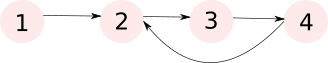
\includegraphics[scale=1.0]{sources/cycle_in_list/images/example1}
	\caption{Example of linked list with a cycle.}
\end{figure}
\begin{figure}
	\label{fig:cycle_in_list:example2}
	\centering
	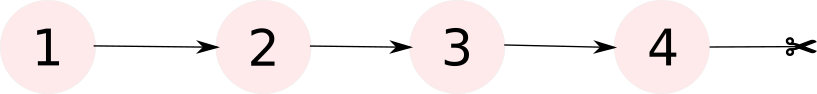
\includegraphics[scale=1.0]{sources/cycle_in_list/images/example2}
	\caption{Example of linked list with no cycle.}
\end{figure}

%\section{Clarification Questions}
%
%\begin{QandA}
%	\item 
%	\begin{answered}
%		\textit{}
%	\end{answered}
%	
%\end{QandA}

\section{Discussion}
\label{cycle_in_list:sec:discussion}
Considering this is a very well known problem we will not spent time on dwelling on naive bruteforce solution, and instead will only concentrate first on a optimal in time time solution with linear space, and then we will concentrate on improving it by lowering the space complexity to constant.

\subsection{Linear time and space solution}
\label{cycle_in_list:sec:bruteforce}
This problem has many similarities with the problem of finding a duplicate in a collection and can therefore be solved using a similar approach. The idea is to visit the list and store in a hash-set the  address of the node \textbf{already} visited. While visiting a new node, we first check if that node was already visited, and if yes, it means that we can stop because we found the starting point of a loop. If we reach the end of the list and we were not be able to find a duplicate, then it means there is no loop and we can return \lstinline[columns=fixed]{nullptr}.
A possible implementation of this idea is shown in Listing \ref{list:cycle_in_list:linearspace}.

\lstinputlisting[language=c++, caption={Linear time and space solution to the problem of detecting a cycle in a linked list.},label=list:cycle_in_list:linearspace]{sources/cycle_in_list/cycle_in_list_solution1.cpp}



\subsection{Slow and fast pointer solution - Floyd’s algorithm }
\label{cycle_in_list:sec:slowfast}
This algorithm\cite{cit::wiki::floyd} uses the fact that, like clock's hands, things iterating on a cycle at different speed will eventually meet at some point in the future. Consider two runner $R_1$ and $R_2$ with velocities $V_1$ and $V_2=2V_1$ respectively ($R_2$ goes twice as fast then $R_1$), starting their run from the same point in a circular stadium. They will meet again when the slower runner reach the starting point for the second time. Why? By the time the slower one has completed half circle the faster has completed a complete cycle and by the time the slower finishes his run, arriving at the starting point again, the faster has completed a second entire cycle. We can use this fact to detect a cycle in a linked list even if for the cycle detection problem things might be a bit more complicated because the two runners might now start going in loop at the same time (the list potentially has a first part the is not part of the loop as can be seen in Figure \ref{fig:cycle_in_list:example1}).
The rest of the section is a bit technical and you can skip to the implementation shown in Listing \ref{list:cycle_in_list:constantspace} which can be self explanatory considering that in the end the intutition behind the algorithm is quite easy. If you are interested in the details of why it works, read along. 

Consider two iterators p,q with velocities $v_p=1$,$v_q=2$  respectively. Suppose the \textbf{cycle}(not the entire list) has length $n$. We can have two scenario depending on the index $A$ of the starting node of the cycle:

\begin{enumerate}
\item the cycle starts at $A < n$.
\item or  starts at \(A \geq n\).
\end{enumerate}

For the case $(1)$ when the slower iterator reaches $A$ the faster is at location $2A$ (which might mean that the faster iterator looped around the cycle already). How many iteration $k$ it will take before they meet? And at which node?

The situation is described by the following congruences:
\begin{align}
  A + kv_p &\equiv 2A + k2v_p \Mod{n} \\
  2A + k2v_p &\equiv A + kv_p \;  \Mod{n} \\
  A + k2v_p &\equiv kv_p   \Mod{n} \\
  A +kv_p &\equiv 0   \Mod{n} \\
  A +k &\equiv 0  \Mod{n}
\end{align}
which has solution \(k = n-A\). This means that they will meet after \(k=n-A\) iterations of the slower iterator, i.e. at \(A\) nodes before the beginning of the cycle and we can use this fact to count \(A\) nodes from the beginning of the list so to find the starting point of the cycle. 

So, once the iterators meet \textbf{in the cycle}, we can move the fast iterator back to the beginning of the list and iterate forward one node per step with both iterators until they match again. When we move the fast iterator back at the head of the list, \textbf{both iterators are \(A\) nodes away from the beginning of the cycle}. Because of this, when we move both of them by one, they will eventually meet exactly at that node \(A\) i.e. the beginning of the cycle.

%%%------------

Let's consider now the case ($2$) i.e.  when \(A \geq n\). This means that by the time the slower iterator reaches the beginning of the cycle the faster one has completed more that a cycle. What will be the starting point for the faster one? We argue that once \(p\) reaches \(A\), \(q\) is at node \(2A\) but since \(A > n\), this means that it will be at position \(A + (A \Mod{n})\). We can now use similar argument to the previous case and write:

\begin{align}
  A + kv_p &\equiv A + (A \Mod{n}) + (k2v_p \Mod{n}) \\
  A + (A \Mod{n}) + k2v_p &\equiv A + kv_p\;\Mod{n} \\
  (A \Mod{n}) + kv_p \Mod{n} & \equiv 0\Mod{n} \\
  (A \Mod{n}) + k \Mod{n} &\equiv 0 \Mod{n} \: \: \text{  : because  } v_p=1 \\
\end{align}


which has solution \(k = n-(A \Mod{n})\). This means that the meeting point is \(A \Mod{n}\) nodes before the beginning of the cycle. If we do the same operations as the previous case,(when \(A < n\)), we obtain again, the same result. Iterators will meet at the beginning of the cycle. Why? Well advancing \(q\) makes \(p\) cycle possibly several times ( remember that \(A \geq n\)  ) and it will clearly stops at \( A+(n-A \Mod{n}) + A \Mod{n} = A +n \;(mod (n))= A\).

In other words the slower pointer is at first  at node number \(A+(n-A \Mod{n})\). We can write \( A = bn + r\) where \(r = A \;\Mod{n}\). After \(A\) advancing steps it will be at location  \( A+(n-A \;\Mod{n}) +bn +r (\Mod{n})\). Since \(bn \; \Mod{n}=0\) the result follows.

As an example consider a list with a cycle of length \(n=4\) starting at node number \(10\). The first part of the algorithm tells us that the nodes will meet at node \(10 + 4 - 10 \: mod(4) = 12\). Moving the fast pointer back to the head of the list and iterating one node per time both iterators will lead the slower point to node:



Figures \ref{fig:cycle_in_list:flow1} and \ref{fig:cycle_in_list:flow2} depict how the algorithm would work on a list of $8$ nodes with a cycle of length $4$ starting at node number $4$. After $5$ steps the slow (blue) and fast (red) iterator points to the same node i.e. node number $6$.
After that the fast pointer is moved to the head of the list and both iterator are incremented by $1$ until they meet again. When they do, they will meet at the beginning of the cycle.
An implementation of the Floyd's algorithm is shown in Listing \ref{list:cycle_in_list:constantspace}.
\lstinputlisting[language=c++, caption={Floyd's algorithm, linear time, constant space solution to the problem of detecting a cycle in a linked list.},label=list:cycle_in_list:constantspace]{sources/cycle_in_list/cycle_in_list_solution2.cpp}


\begin{figure}[htbp]
	\label{fig:cycle_in_list:flow1}
	\centering
	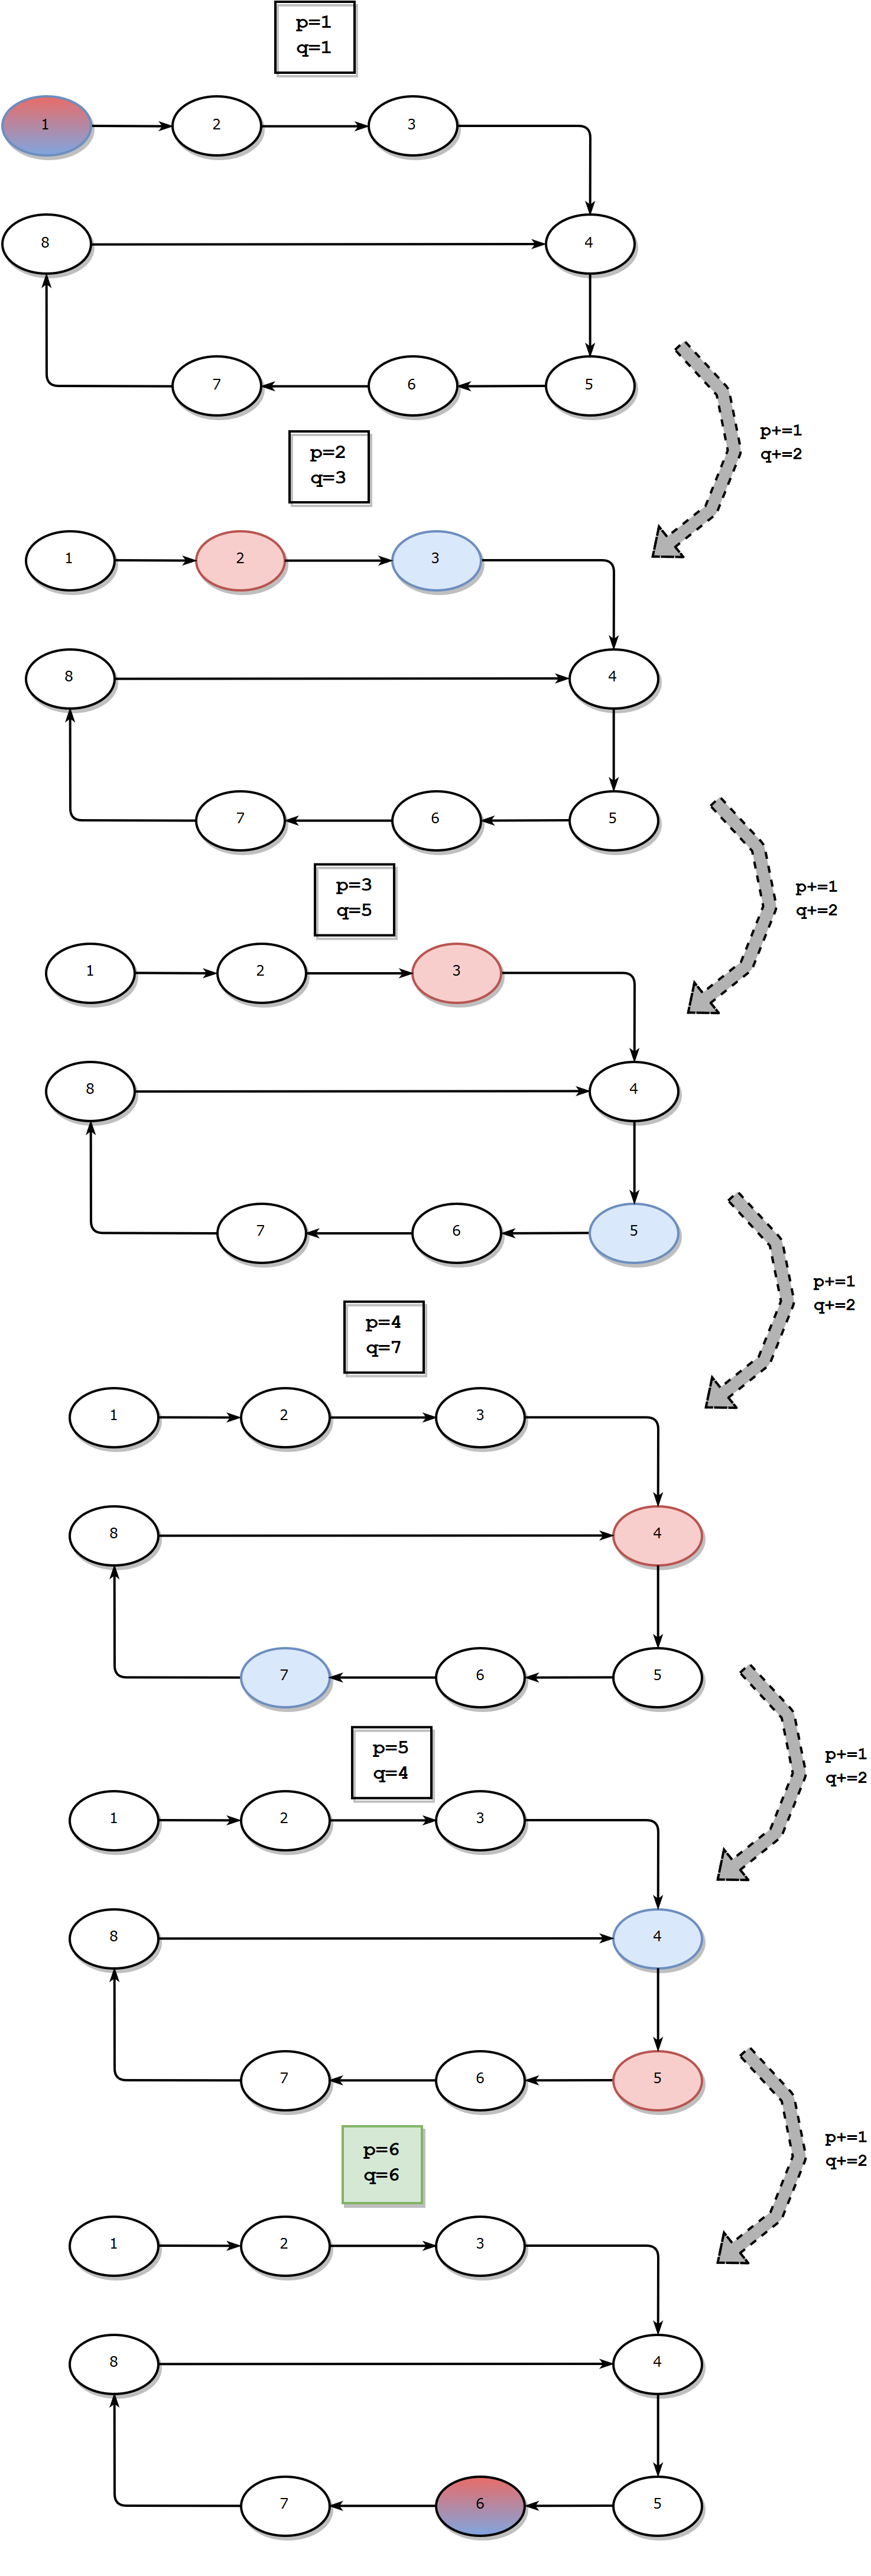
\includegraphics[scale=0.15]{sources/cycle_in_list/images/flow1}
	\caption{Execution of the first phase of the Floyd's algorithm on a list of $8$ nodes with a cycle of length $4$ starting at node $4$.}
\end{figure}

\begin{figure}[htbp]
	\label{fig:cycle_in_list:flow2}
	\centering
	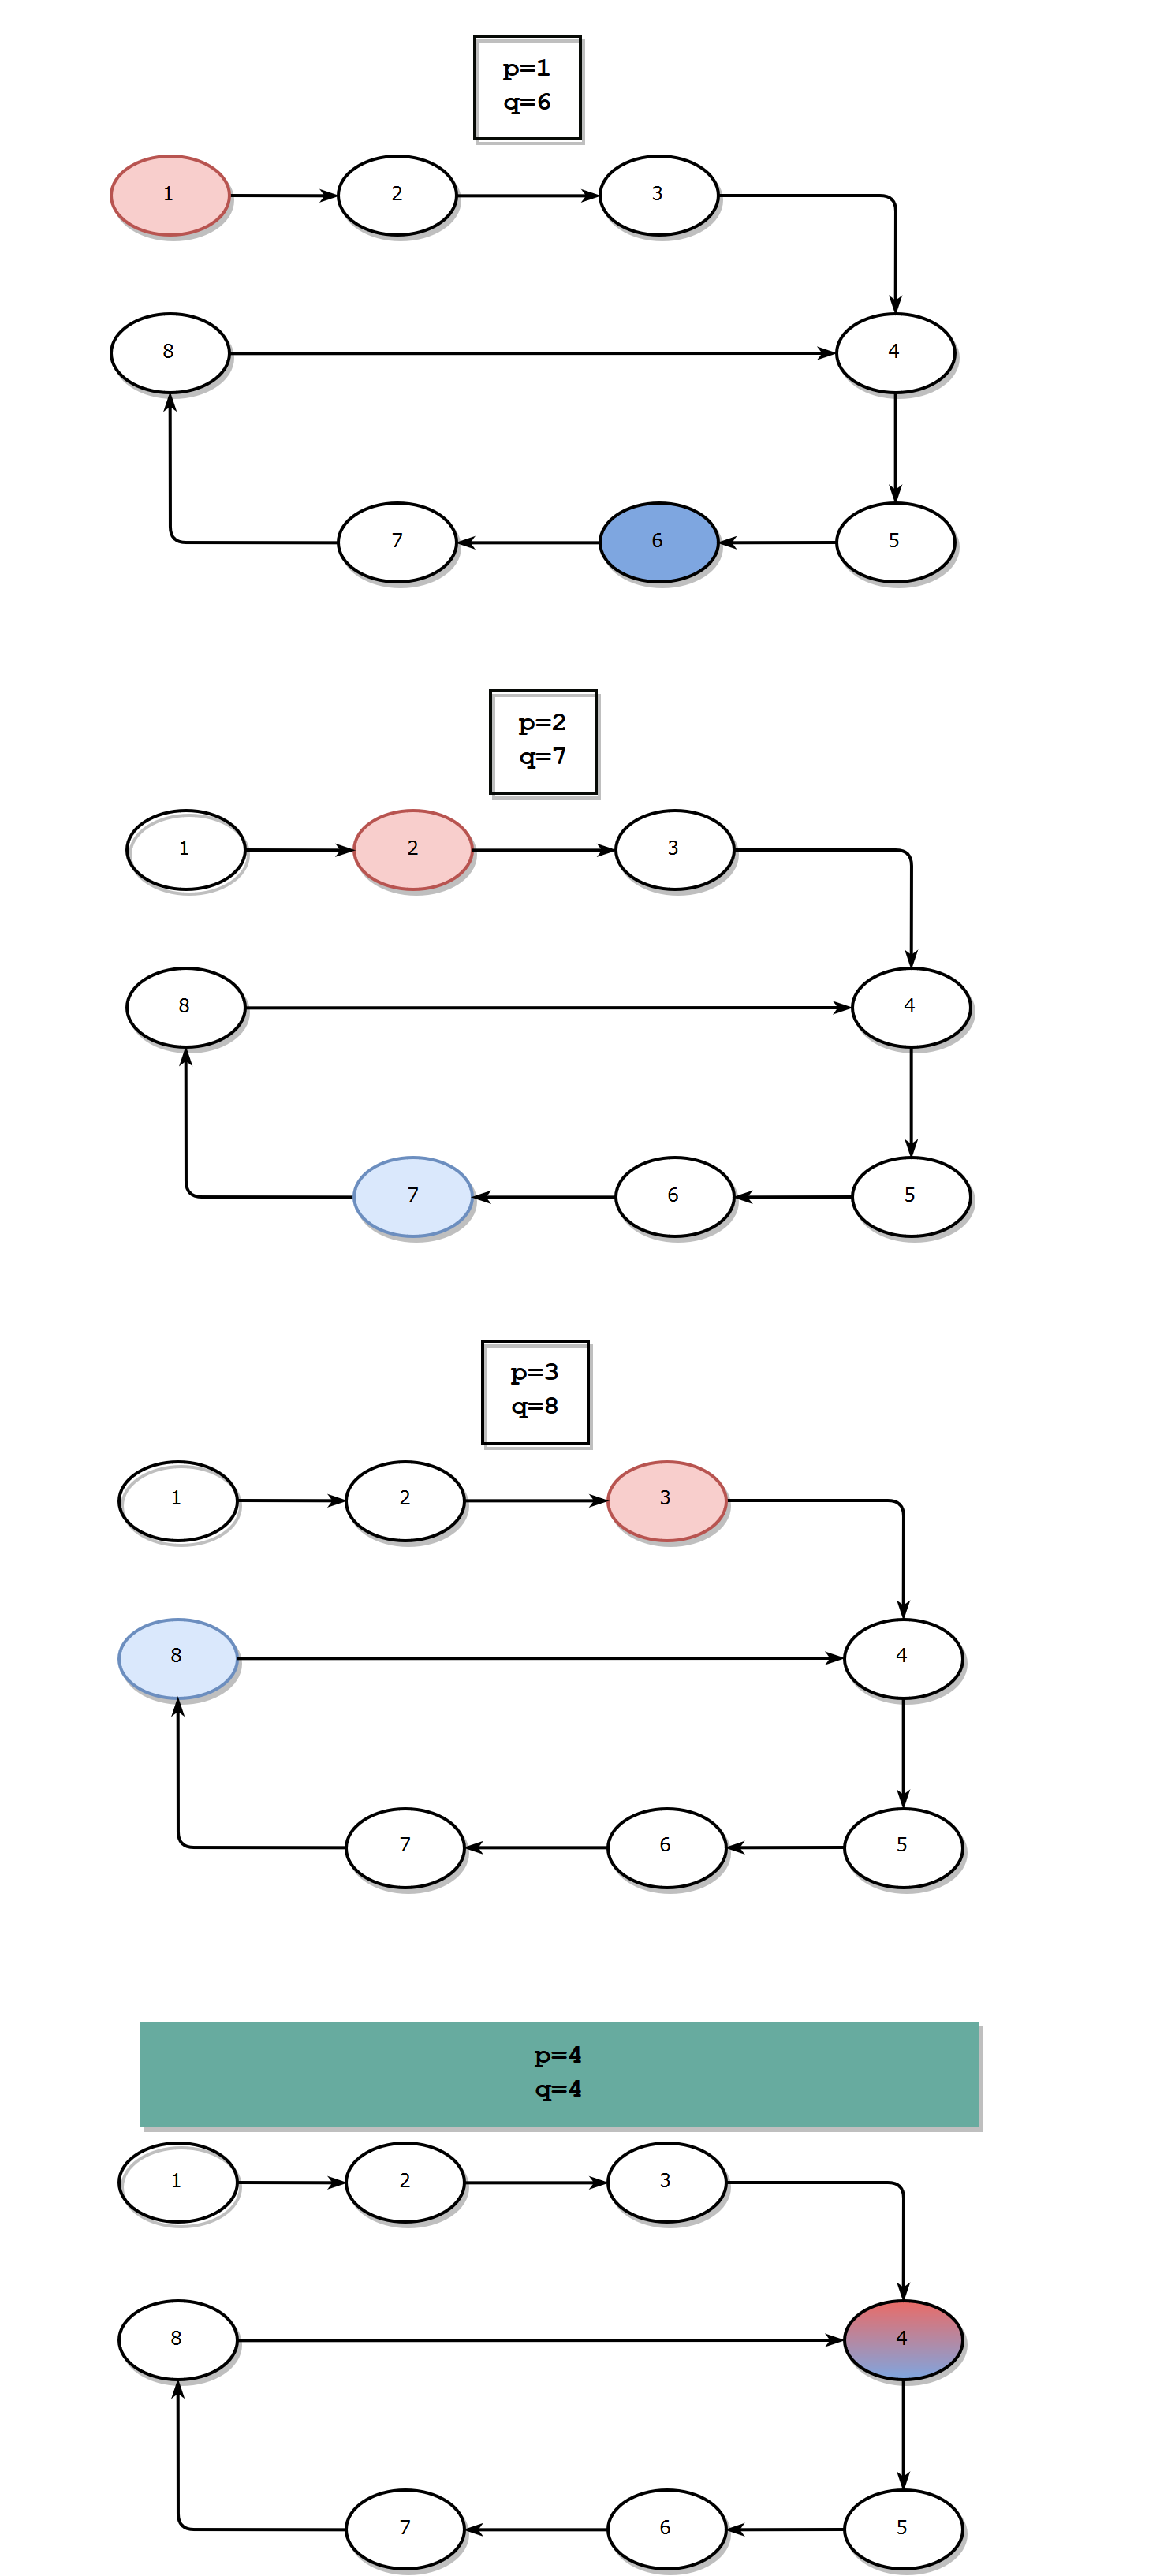
\includegraphics[scale=0.15]{sources/cycle_in_list/images/flow2}
	\caption{Execution of the second phase of the Floyd's algorithm on a list of $8$ nodes with a cycle of length $4$ starting at node $4$.}
\end{figure}
